\documentclass[aspectratio=169,11pt]{beamer}
\usepackage[utf8]{inputenc}
\usepackage[T1]{fontenc}
\usepackage{helvet}
\usepackage{tikz}
\usepackage{booktabs}
\usepackage{array}
\usetikzlibrary{arrows.meta,positioning,shapes.misc,calc}

% ---- palette: matches the app ----
\definecolor{ivory}{HTML}{FAF9F5}
\definecolor{ink}{HTML}{1F1E1B}
\definecolor{muted}{HTML}{6E6B63}
\definecolor{clay}{HTML}{C96442}
\definecolor{clayd}{HTML}{B25638}
\definecolor{line}{HTML}{E4E1D7}
\definecolor{card}{HTML}{FFFFFF}
\definecolor{okg}{HTML}{0B6B3A}
% ---- game-world dark variant ----
\definecolor{night}{HTML}{15131C}
\definecolor{plight}{HTML}{B7B3A8}
\definecolor{gold}{HTML}{E0B45C}

\setbeamercolor{background canvas}{bg=ivory}
\setbeamercolor{normal text}{fg=ink}
\setbeamercolor{structure}{fg=clay}
\setbeamercolor{frametitle}{fg=ink,bg=ivory}
\setbeamercolor{title}{fg=ink}
\setbeamerfont{frametitle}{family=\rmfamily,size=\Large,series=\mdseries}
\setbeamerfont{title}{family=\rmfamily,size=\Huge,series=\mdseries}
\setbeamertemplate{navigation symbols}{}
\setbeamertemplate{itemize item}{\textcolor{clay}{\rule[0.4ex]{0.7ex}{0.7ex}}}
\setbeamertemplate{itemize subitem}{\textcolor{muted}{--}}
\setbeamertemplate{frametitle}{\vspace{0.8em}\usebeamerfont{frametitle}\insertframetitle\par\vspace{0.15em}{\color{line}\hrule height 1pt}\vspace{0.2em}}
\setbeamertemplate{footline}{\hfill{\color{muted}\scriptsize\insertframenumber\hspace{2em}}\vspace{0.6em}}

\newcommand{\kicker}[1]{{\color{clay}\scriptsize\bfseries\MakeUppercase{#1}}\\[0.3em]}
\newcommand{\mutedtext}[1]{{\color{muted}#1}}
\newcommand{\dmuted}[1]{{\color{plight}#1}}
% wrap dark game frames in \begin{darkslides}...\end{darkslides}
\newenvironment{darkslides}{%
  \setbeamercolor{background canvas}{bg=night}%
  \setbeamercolor{normal text}{fg=ivory}%
  \setbeamercolor{frametitle}{fg=ivory,bg=night}%
  \setbeamercolor{title}{fg=ivory}%
  \setbeamercolor{itemize/enumerate body}{fg=ivory}%
  \setbeamercolor{itemize/enumerate subbody}{fg=plight}%
}{}

\title{Prometheus Lab}
\author{}
\date{}

\begin{document}

% ---------------------------------------------------------------- 1 TITLE (dark)
\begin{darkslides}
\begin{frame}
  \color{ivory}
  \begin{center}
    \vspace{1.2em}
    \kicker{GDG Windsor · Build with AI · Edge / On-Device Track}
    {\rmfamily\fontsize{34}{38}\selectfont\color{ivory} Prometheus Lab\par}
    \vspace{0.6em}
    {\large An on-device math adventure for the Grade 9 EQAO.\par}
    \vspace{0.4em}
    \dmuted{Five monsters guard the Citadel. Each one is a trick --- a wrong idea that feels right.\\ Defeat the idea, and the golden gate opens. Nothing ever leaves the laptop.}\par
    \vspace{1.6em}
    {\small Gokulakrishnan \,·\, Padmanabha \,·\, Taha \,·\, Naimah \,·\, Amarah}
  \end{center}
\end{frame}
\end{darkslides}

% ---------------------------------------------------------------- 2 PROBLEM
\begin{frame}{The problem: wrong answers are symptoms, not causes}
  \begin{columns}[T]
    \begin{column}{0.55\textwidth}
      \begin{itemize}\setlength\itemsep{0.7em}
        \item Every Ontario Grade 9 student writes the EQAO math assessment. Many arrive with \textbf{specific, well-documented tricks} --- wrong ideas that feel right, not general weakness.
        \item A student who answers $\tfrac{2}{3}+\tfrac{1}{4}=\tfrac{3}{7}$ doesn't need more practice. They need someone to notice they \textbf{add tops and bottoms straight across} --- and fix exactly that.
        \item Teachers can't do this per-student, per-trick. \textbf{So we turned each trick into a monster you can fight.}
      \end{itemize}
    \end{column}
    \begin{column}{0.42\textwidth}
      \begin{tikzpicture}[scale=0.9]
        \node[draw=line, fill=card, rounded corners=2pt, inner sep=8pt, text width=5.2cm, align=left] at (0,0) {
          {\small Calculate $\tfrac{2}{3}+\tfrac{1}{4}$}\\[3pt]
          {\small A) $\tfrac{11}{12}$ \hfill {\color{okg}\scriptsize correct}}\\[2pt]
          {\small \textbf{B) $\tfrac{3}{7}$} \hfill {\color{clay}\scriptsize adds straight across}}\\[2pt]
          {\small C) $\tfrac{3}{12}$ \hfill {\color{muted}\scriptsize didn't rescale tops}}\\[2pt]
          {\small D) $\tfrac{11}{7}$ \hfill {\color{muted}\scriptsize mixed method}}\\[4pt]
          {\scriptsize\color{muted} Every wrong option is the exact result of a \emph{known} trick --- so the wrong answer itself is the diagnosis.}
        };
      \end{tikzpicture}
    \end{column}
  \end{columns}
\end{frame}

% ---------------------------------------------------------------- 3 GAME WORLD (dark)
\begin{darkslides}
\begin{frame}{The game world: the Citadel}
  \color{ivory}
  {\small A gothic castle nexus in three.js --- drag to orbit. Five monsters idle on floating platforms, each guarding one curriculum strand and a sealed \textcolor{gold}{golden gate}. Someone is locked in the keep; defeat all five to open it.}\par
  \vspace{0.2em}
  \renewcommand{\arraystretch}{1.15}
  {\footnotesize
  \begin{tabular}{@{}p{2.1cm}>{\raggedright\arraybackslash}p{3.6cm}p{7.2cm}@{}}
    \toprule
    \textbf{Monster} & \textbf{Strand (MTH1W)} & \textbf{The trick it feeds on} \\
    \midrule
    Fractis    & Number                  & adding fractions straight across, tops and bottoms \\
    Equazor    & Algebra                 & signs that slip when balancing an equation \\
    Statiq     & Data                    & mean and median blurred into the same idea \\
    Polygor    & Geometry \& Measurement & formulas that are \emph{almost} right \\
    Ledgerling & Financial Literacy      & interest skimmed off a sloppy budget \\
    \bottomrule
  \end{tabular}}
  \vspace{0.2em}
  \begin{itemize}\setlength\itemsep{0.2em}
    \item {\small The game captures your \textbf{hero name}; monsters address you by it in full-screen encounter cinematics.}
    \item {\small And they \textbf{remember}: Gemma writes each monster's greeting from your actual battle history.}
  \end{itemize}
\end{frame}
\end{darkslides}

% ---------------------------------------------------------------- 4 PLAYER JOURNEY
\begin{frame}{The player journey}
  \begin{center}
  \resizebox{\textwidth}{!}{%
  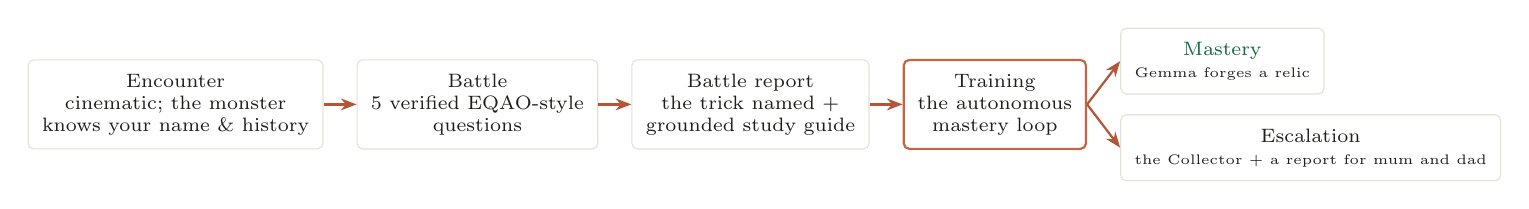
\begin{tikzpicture}[
      node distance=0.45cm and 0.42cm,
      box/.style={draw=line, fill=card, rounded corners=2pt, inner sep=5pt, align=center, font=\scriptsize, text=ink},
      accent/.style={draw=clay, thick, fill=card, rounded corners=2pt, inner sep=5pt, align=center, font=\scriptsize, text=ink},
      arr/.style={-{Stealth[length=2mm]}, thick, color=clayd}]
    \node[box] (enc) {Encounter\\ \scriptsize cinematic; the monster\\ \scriptsize knows your name \& history};
    \node[box, right=of enc] (battle) {Battle\\ \scriptsize 5 verified EQAO-style\\ \scriptsize questions};
    \node[box, right=of battle] (report) {Battle report\\ \scriptsize the trick named +\\ \scriptsize grounded study guide};
    \node[accent, right=of report] (train) {Training\\ \scriptsize the autonomous\\ \scriptsize mastery loop};
    \node[box, above right=0.55cm and 0.42cm of train.east, anchor=west] (win) {\color{okg}Mastery\\ \tiny Gemma forges a relic};
    \node[box, below right=0.55cm and 0.42cm of train.east, anchor=west] (esc) {Escalation\\ \tiny the Collector + a report for mum and dad};
    \draw[arr] (enc) -- (battle);
    \draw[arr] (battle) -- (report);
    \draw[arr] (report) -- (train);
    \draw[arr] (train.east) -- (win.west);
    \draw[arr] (train.east) -- (esc.west);
  \end{tikzpicture}}
  \end{center}
  \vspace{0.4em}
  \begin{itemize}\setlength\itemsep{0.4em}
    \item Miss a question and the agent reads the wrong option's tag, names the \textbf{exact trick}, and builds a study guide grounded in the verified solution --- with real exponent and fraction notation on screen.
    \item Then it \textbf{pursues a goal}: keep teaching, with different strategies, until you \emph{demonstrate} the trick is gone --- or the Collector comes for you.
  \end{itemize}
\end{frame}

% ---------------------------------------------------------------- 5 AGENT LOOP
\begin{frame}{An agent, not a chatbot}
  \begin{columns}[T]
    \begin{column}{0.56\textwidth}
      \begin{center}
      \resizebox{\columnwidth}{!}{%
      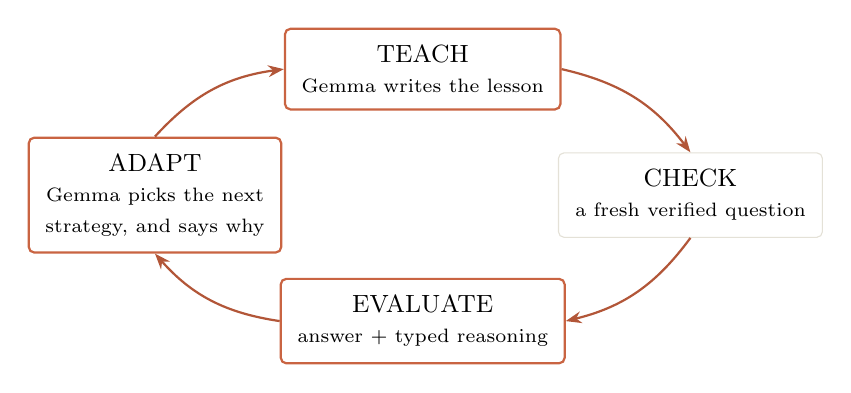
\begin{tikzpicture}[
          box/.style={draw=line, fill=card, rounded corners=2pt, inner sep=6pt, align=center, font=\small, minimum width=2.6cm},
          gbox/.style={draw=clay, thick, fill=card, rounded corners=2pt, inner sep=6pt, align=center, font=\small, minimum width=2.6cm},
          arr/.style={-{Stealth[length=2mm]}, thick, color=clayd}]
        \node[gbox] (teach) at (0,2.4) {TEACH\\ \scriptsize Gemma writes the lesson};
        \node[box] (check) at (3.4,0.8) {CHECK\\ \scriptsize a fresh verified question};
        \node[gbox] (eval) at (0,-0.8) {EVALUATE\\ \scriptsize answer + typed reasoning};
        \node[gbox] (adapt) at (-3.4,0.8) {ADAPT\\ \scriptsize Gemma picks the next\\ \scriptsize strategy, and says why};
        \draw[arr] (teach.east) to[bend left=20] (check.north);
        \draw[arr] (check.south) to[bend left=20] (eval.east);
        \draw[arr] (eval.west) to[bend left=20] (adapt.south);
        \draw[arr] (adapt.north) to[bend left=20] (teach.west);
      \end{tikzpicture}}
      \end{center}
    \end{column}
    \begin{column}{0.42\textwidth}
      {\small \textbf{The reasoning gate:} a right answer with shaky typed reasoning \textbf{does not count} --- Gemma grades the explanation (closed labels), not just the bubble.\par
      \vspace{0.5em}
      \textbf{Explainable everywhere:} every decision shows its why --- \mutedtext{``Trying a visual walkthrough --- you said you can't see why the denominators matter.''}\par
      \vspace{0.5em}
      \textbf{It cannot run away:} 4-attempt cap, 12-model-call budget, exhaustion $\rightarrow$ clean hand-off.\par}
      \vspace{0.3em}
      {\scriptsize\color{muted}Orange boxes = Gemma. Every session provably terminates.}
    \end{column}
  \end{columns}
\end{frame}

% ---------------------------------------------------------------- 6 GEMMA ROLES
\begin{frame}{Where Gemma does the thinking \hfill {\normalsize\color{muted}rubric: Gemma Integration, 30\%}}
  \renewcommand{\arraystretch}{1.15}
  {\scriptsize
  \begin{tabular}{@{}p{4.0cm}p{9.3cm}@{}}
    \toprule
    \textbf{Gemma's job (8 call sites)} & \textbf{Guardrail} \\
    \midrule
    Write the lesson \& study guide & grounded in the verified solution; explains \emph{why}, never recomputes \\
    Grade typed reasoning & closed labels; fail-open --- never punishes the student \\
    Choose the next strategy & limited to the remaining ladder; states its rationale; code fallback \\
    Author fresh check questions & bank-first; must pass a blind self-solve audit or is discarded \\
    Monster memory lines & one line, from real battle history; scripted fallback \\
    Forge the mastery relic & flavour only --- the facts are injected by code \\
    Write the mum-and-dad report & narrative only; every number comes from the session log \\
    Coach the speed trials & reads miss + latency telemetry; names the pattern; sets a 3-question drill \\
    \bottomrule
  \end{tabular}}
  \vspace{0.25em}
  \begin{itemize}\setlength\itemsep{0.15em}
    \item {\small Remove Gemma and there is no game. \textbf{But the math truth never depends on it.}}
    \item {\small One auditable door (\texttt{gemma\_client.py}); model size is a dial: \texttt{gemma4:12b} primary, \texttt{gemma4:1b} light.}
  \end{itemize}
\end{frame}

% ---------------------------------------------------------------- 7 COLLECTOR (dark)
\begin{darkslides}
\begin{frame}{The Collector, his lieutenants, and the Gemma coach}
  \color{ivory}
  \begin{columns}[T]
    \begin{column}{0.5\textwidth}
      \textbf{\textcolor{gold}{THE COLLECTOR}} --- {\small a giant skull boss, summoned when the mastery loop escalates: a mental-math speed trial, 3 lives, he attacks on every miss. Gemma writes the report for mum and dad alongside --- the agent knows its limits.}\par
      \vspace{0.2em}
      \textbf{Three lieutenants}, one mental-math lane each:
      \begin{itemize}\setlength\itemsep{0.2em}
        \item {\small \textbf{Twinfang} --- doubles and halves}
        \item {\small \textbf{The Niner} --- the nines shortcut}
        \item {\small \textbf{Splitjaw} --- make-a-ten}
      \end{itemize}
      {\small 90-second war-clock skirmishes with streak escalation; every miss and its latency logged.}
    \end{column}
    \begin{column}{0.47\textwidth}
      \textbf{GET COACHED BY GEMMA}
      \begin{itemize}\setlength\itemsep{0.3em}
        \item {\small Before the fight, Gemma \textbf{whispers the lane's mental strategy} in its own words.}
        \item {\small After it, Gemma reads the miss + latency telemetry, \textbf{names your miss pattern}, teaches the fix, and sets a \textbf{3-question drill}.}
        \item {\small The battle is pure client-side speed; \textbf{the coaching is where the model earns its keep}.}
      \end{itemize}
      \vspace{0.15em}
      \dmuted{\scriptsize The whole wing runs to a procedural WebAudio soundscape --- no audio files shipped.}
    \end{column}
  \end{columns}
\end{frame}
\end{darkslides}

% ---------------------------------------------------------------- 8 RELIABILITY
\begin{frame}{We caught our model failing --- and engineered around it}
  \mutedtext{Every guardrail exists because live testing broke something. The commit history is the proof of work.}\par
  \vspace{0.3em}
  \renewcommand{\arraystretch}{1.1}
  {\small
  \begin{tabular}{@{}p{5.8cm}>{\raggedright\arraybackslash}p{7.2cm}@{}}
    \toprule
    \textbf{Caught in testing} & \textbf{Architectural fix} \\
    \midrule
    Generated a question with a \textbf{wrong answer key} & blind self-solve audit; bank-first check questions \\
    Wrote a check question \textbf{in Spanish} & constrained generation prompts \\
    \textbf{Invented wrong arithmetic} in an explanation ($\tfrac{2}{3}+\tfrac{1}{4}=\tfrac{17}{12}$) & grounding rule: explain \emph{why}, never recompute; numbers only from the verified solution \\
    Rambled when reconstructing multi-step errors & diagnosis by ground-truth tag lookup, not model reasoning \\
    Emitted \texttt{2\^{}3} and \texttt{2/3} as raw markup & notation layer: real exponents and stacked fractions on screen \\
    \bottomrule
  \end{tabular}}
  \vspace{0.25em}
  \begin{itemize}
    \item {\small The result: \textbf{the model is never the source of truth for math} anywhere a student can see it.}
  \end{itemize}
\end{frame}

% ---------------------------------------------------------------- 9 EDGE
\begin{frame}{Fully on-device \hfill {\normalsize\color{muted}the Edge track promise, kept literally}}
  \begin{columns}[T]
    \begin{column}{0.55\textwidth}
      \begin{itemize}\setlength\itemsep{0.3em}
        \item {\small Gemma runs locally via \textbf{Ollama}: \texttt{gemma4:12b} primary, \texttt{gemma4:1b} light --- one env var. Works in airplane mode.}
        \item {\small The 3D world is local too: \textbf{three.js and the CC0 Quaternius monsters are vendored} --- no CDN.}
        \item {\small The soundscape is \textbf{synthesized procedurally in WebAudio} --- zero audio files.}
        \item {\small A student's struggles are a protected record --- \textbf{they stay on their machine.}}
      \end{itemize}
      {\scriptsize\color{muted}Companion Kaggle notebook: Gemma 4 12b-it on a cloud GPU --- the app never leaves the laptop.}
    \end{column}
    \begin{column}{0.42\textwidth}
      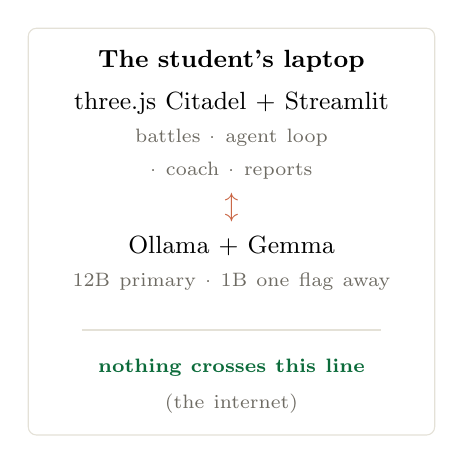
\begin{tikzpicture}
        \node[draw=line, fill=card, rounded corners=3pt, inner sep=8pt, text width=4.6cm, align=center] {
          {\small\bfseries The student's laptop}\\[3pt]
          {\small three.js Citadel + Streamlit}\\
          {\scriptsize\color{muted}battles · agent loop · coach · reports}\\[2pt]
          {\color{clay}$\updownarrow$}\\[2pt]
          {\small Ollama + Gemma}\\
          {\scriptsize\color{muted}12B primary · 1B one flag away}\\[4pt]
          {\color{line}\rule{3.8cm}{0.6pt}}\\[3pt]
          {\scriptsize\color{okg}\bfseries nothing crosses this line}\\[1pt]
          {\scriptsize\color{muted}(the internet)}
        };
      \end{tikzpicture}
    \end{column}
  \end{columns}
\end{frame}

% ---------------------------------------------------------------- 10 DEMO
\begin{frame}{The 90-second live demo}
  \begin{enumerate}\setlength\itemsep{0.4em}
    \item {\small \textbf{The Citadel} --- drag the castle; five monsters idle on their platforms; the keep is sealed.}
    \item {\small \textbf{Encounter} --- Fractis addresses us by our hero name and \emph{remembers our last visit}.}
    \item {\small \textbf{The miss} --- we add $\tfrac{2}{3}+\tfrac{1}{4}$ straight across; the battle report names the exact trick.}
    \item {\small \textbf{The agent adapts} --- we answer wrong \emph{and type our flawed reasoning}; the agent switches strategy \textbf{and explains why}, live on screen.}
    \item {\small \textbf{The relic} --- two fresh correct answers with solid reasoning $\rightarrow$ Gemma forges our trophy.}
    \item {\small \textbf{The Collector's wing} --- a 90-second lieutenant skirmish, then \textbf{GET COACHED BY GEMMA}: it reads our misses, names the pattern, and drills the fix.}
  \end{enumerate}
  \vspace{0.25em}
  \mutedtext{\small Everything shown runs live on this laptop. Wi-Fi can be off.}
\end{frame}

% ---------------------------------------------------------------- 11 ROADMAP
\begin{frame}{What's next \hfill {\normalsize\color{muted}same architecture, deeper world}}
  \begin{itemize}\setlength\itemsep{0.6em}
    \item \textbf{Local tool use} --- Gemma emits constrained JSON tool calls; a local SymPy verifier proves every answer deterministically. \mutedtext{\small (tool use for a model that doesn't natively support it)}
    \item \textbf{Beyond the golden gate} --- the rescue arc continues: new keeps, new boss lanes, harder relics --- same agent brain underneath.
    \item \textbf{Classroom mode} --- session records roll up across a whole class, still local-first: the school's data stays in the school.
  \end{itemize}
  \vspace{0.7em}
  {\color{line}\hrule height 1pt}
  \vspace{0.5em}
  \kicker{How we score ourselves on the rubric}
  \resizebox{\textwidth}{!}{%
  \begin{tabular}{@{}llll@{}}
    \textbf{Gemma Integration 30\%} & \textbf{Innovation 30\%} & \textbf{Functionality 20\%} & \textbf{Writeup 20\%} \\
    \mutedtext{\scriptsize 8 roles, all guardrailed} & \mutedtext{\scriptsize a tutor agent you can fight} & \mutedtext{\scriptsize live, on-device, terminates} & \mutedtext{\scriptsize honest engineering story} \\
  \end{tabular}}
\end{frame}

% ---------------------------------------------------------------- 12 CLOSE (dark)
\begin{darkslides}
\begin{frame}
  \color{ivory}
  \begin{center}
    \vspace{1.5em}
    {\rmfamily\fontsize{26}{32}\selectfont\color{ivory} Every monster is a trick ---\\ a wrong idea that feels right.\par}
    \vspace{1.0em}
    {\rmfamily\large\color{gold} Defeat the idea, and the gate opens.\par}
    \vspace{1.2em}
    \dmuted{\small A student walks in adding fractions straight across. Twenty minutes later they've \emph{proven} the trick is gone --- and nothing about them ever left their laptop.}\par
    \vspace{1.4em}
    \dmuted{\small github.com/EdTechDL/gemma-without-borders \,·\, live demo + clonable notebook}\par
    \vspace{0.5em}
    {\small Gokulakrishnan \,·\, Padmanabha \,·\, Taha \,·\, Naimah \,·\, Amarah}
  \end{center}
\end{frame}
\end{darkslides}

\end{document}
